\documentclass[preview]{standalone}

\usepackage{amsmath}
\usepackage{amssymb}
\usepackage{tikz}
\usepackage{stellar}
\usepackage{definitions}
\usepackage{bettelini}

\begin{document}

\id{linearalgebra-subspaces}
\genpage

\section{Linear subspaces}

\begin{snippetdefinition}{linear-subspace-definition}{Linear subspace}
    Let \(V\) be a \vectorspace over a \field \(\mathbb{F}\). A
    \emph{linear subspace} of \(V\) is a \set \(U\subseteq V\) such that
    \(U\), with the vector addition and scalar multiplication inherited from
    \(V\), is a \vectorspace over \(\mathbb{F}\).
\end{snippetdefinition}

\begin{snippet}{linear-subspace-stability-idea}
    A linear subspace is a part of a \vectorspace that is stable under the
    \vectorspace operations: adding two \vector[vectors] of the subspace stays in the
    subspace, and multiplying a \vector of the subspace by a \vsscalar stays in
    the subspace.
\end{snippet}

\begin{snippettheorem}{linear-subspace-criterion-theorem}{Linear subspace criterion}
    Let \(V\) be a \vectorspace over a \field \(\mathbb{F}\), and let
    \(U\subseteq V\). Then \(U\) is a linear subspace of \(V\) \ifandonlyif
    \begin{enumerate}
        \item \(0_V\in U\);
        \item \(u,v\in U \implies u+v\in U\);
        \item \(\lambda\in\mathbb{F}, u\in U \implies \lambda u\in U\).
    \end{enumerate}
\end{snippettheorem}

\begin{snippetproof}{linear-subspace-criterion-theorem-proof}{linear-subspace-criterion-theorem}{Linear subspace criterion}
    \begin{iffproof}
        \item Suppose that \(U\) is a linear subspace of \(V\). Since \(U\)
        is a \vectorspace, it contains its zero \vector. Because the operations
        are inherited from \(V\), this zero \vector is \(0_V\). Addition and
        scalar multiplication are internal operations on \(U\), so conditions
        \(2\) and \(3\) hold.

        \item Suppose that the three conditions hold. Then addition and
        scalar multiplication restrict to operations
        \[
            +\colon U\cartesianprod U\fromto U,
            \qquad
            \cdot\colon \mathbb{F}\cartesianprod U\fromto U.
        \]
        All \vectorspace identities hold in \(U\) because they already hold
        in \(V\). The first condition gives the additive identity. If
        \(u\in U\), then \(-u=(-1)u\in U\) by closure under scalar
        multiplication. Hence every element of \(U\) has its additive inverse
        in \(U\). Therefore \(U\) is a \vectorspace over \(\mathbb{F}\).
    \end{iffproof}
\end{snippetproof}

\section{Examples}

\begin{snippetexample}{coordinate-plane-linear-subspace-example}{A coordinate plane in \(F^3\)}
    Let \(V=\mathbb{F}^3\) and
    \[
        U=\{(x_1,x_2,0)\suchthat x_1,x_2\in\mathbb{F}\}.
    \]
    Then \(U\) is a linear subspace of \(\mathbb{F}^3\). Indeed,
    \(0=(0,0,0)\in U\). If
    \[
        u=(x_1,x_2,0),
        \qquad
        v=(y_1,y_2,0),
    \]
    then
    \[
        u+v=(x_1+y_1,x_2+y_2,0)\in U.
    \]
    If \(\lambda\in\mathbb{F}\), then
    \[
        \lambda u=(\lambda x_1,\lambda x_2,0)\in U.
    \]
    By the linear subspace criterion, \(U\) is a linear subspace.
\end{snippetexample}

\begin{snippetexample}{unit-circle-not-linear-subspace-example}{The unit circle is not a linear subspace}
    Let
    \[
        S^1=\{(x,y)\in\realnumbers^2\suchthat x^2+y^2=1\}.
    \]
    This is not a linear subspace of \(\realnumbers^2\). The \vector
    \[
        v=\left(\frac{1}{\sqrt{2}},\frac{1}{\sqrt{2}}\right)
    \]
    belongs to \(S^1\), but
    \[
        2v=(\sqrt{2},\sqrt{2})
    \]
    does not, since
    \[
        (\sqrt{2})^2+(\sqrt{2})^2=4\neq1.
    \]
    Thus \(S^1\) is not closed under scalar multiplication.
    \[
        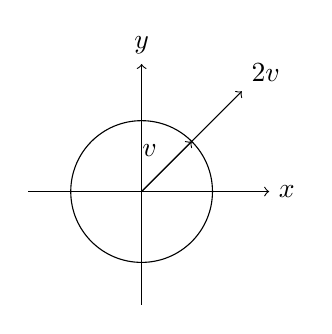
\begin{tikzpicture}[scale=0.9]
            \draw[->] (-1.6,0) -- (1.8,0) node[right] {\(x\)};
            \draw[->] (0,-1.6) -- (0,1.8) node[above] {\(y\)};
            \draw (0,0) circle (1);
            \draw[->] (0,0) -- (0.707,0.707) node[midway, above left] {\(v\)};
            \draw[->] (0,0) -- (1.414,1.414) node[above right] {\(2v\)};
        \end{tikzpicture}
    \]
\end{snippetexample}

\begin{snippetexample}{rationals-subspace-depends-on-scalars-example}{The scalar field matters}
    The real numbers \(\realnumbers\) are a \vectorspace over
    \(\rationalnumbers\). In this \vectorspace,
    \[
        \rationalnumbers\subseteq\realnumbers
    \]
    is a linear subspace: sums of rational numbers are rational, and rational
    multiples of rational numbers are rational.

    The same \set \(\rationalnumbers\) is not a linear subspace of
    \(\realnumbers\) when \(\realnumbers\) is viewed as a \vectorspace over
    \(\realnumbers\). Indeed,
    \[
        1\in\rationalnumbers,
        \qquad
        \sqrt{2}\in\realnumbers,
    \]
    but
    \[
        \sqrt{2}\cdot1=\sqrt{2}\notin\rationalnumbers.
    \]
\end{snippetexample}

\begin{snippetexample}{parameter-subspace-f4-example}{A parameterized subset of \(F^4\)}
    Let
    \[
        U_b=\{(x_1,x_2,x_3,x_4)\in\mathbb{F}^4\suchthat x_3=5x_4+b\}.
    \]
    Then \(U_b\) is a linear subspace of \(\mathbb{F}^4\) if and only if
    \(b=0\). Indeed, a linear subspace must contain the zero \vector, and
    \[
        (0,0,0,0)\in U_b
        \iff
        0=5\cdot0+b
        \iff
        b=0.
    \]
    If \(b=0\), then
    \[
        U_0=\{(x_1,x_2,5t,t)\suchthat x_1,x_2,t\in\mathbb{F}\}.
    \]
    This \set is closed under addition and scalar multiplication, so it is a
    linear subspace.
\end{snippetexample}

\begin{snippetexample}{polynomials-vanishing-at-point-subspace-example}{Polynomials vanishing at a point}
    Let
    \[
        U=\{p\in\realnumbers[x]\suchthat p(5)=0\}.
    \]
    Then \(U\) is a linear subspace of \(\realnumbers[x]\). The zero
    \polynomial belongs to \(U\). If \(p,q\in U\), then
    \[
        (p+q)(5)=p(5)+q(5)=0.
    \]
    If \(\lambda\in\realnumbers\) and \(p\in U\), then
    \[
        (\lambda p)(5)=\lambda p(5)=0.
    \]
\end{snippetexample}

\begin{snippetexample}{trace-zero-matrices-subspace-example}{Trace-zero matrices}
    Let
    \[
        U=
        \left\{
            \begin{pmatrix}
                a & b\\
                c & d
            \end{pmatrix}
            \in\matrices_{2\times2}(\realnumbers)
            \suchthat
            a+d=0
        \right\}.
    \]
    Then \(U\) is a linear subspace of
    \(\matrices_{2\times2}(\realnumbers)\). The zero \matrix belongs to
    \(U\). If \(A=(a_{ij})\) and \(B=(b_{ij})\) have trace \(0\), then
    \(A+B\) has trace \(0\). If \(\lambda\in\realnumbers\), then
    \(\lambda A\) has trace \(\lambda\operatorname{tr}(A)=0\).
\end{snippetexample}

\begin{snippetexample}{r2-linear-subspaces-example}{Linear subspaces of \(\mathbb{R}^2\)}
    The linear subspaces of \(\realnumbers^2\) include
    \[
        \{(0,0)\},
        \qquad
        \realnumbers^2,
    \]
    and every line through the origin. A line that does not pass through the
    origin is not a linear subspace, because it does not contain \(0\).
    \[
        \begin{tikzpicture}[scale=0.9]
            \draw[->] (-2,0) -- (2.5,0) node[right] {\(x\)};
            \draw[->] (0,-1.7) -- (0,2) node[above] {\(y\)};
            \draw (-1.7,-1.1) -- (2,1.3) node[right] {\(U\)};
            \draw (-1.7,1.2) node[below] {\(\text{not a subspace}\)} -- (2.2,1.2);
            \fill (0,0) circle (1.4pt) node[below right] {\(0\)};
        \end{tikzpicture}
    \]
\end{snippetexample}

\begin{snippetexample}{continuous-functions-subspace-example}{Continuous functions}
    Let
    \[
        \mathcal{C}([0,1])
        =
        \{f\colon[0,1]\fromto\realnumbers\suchthat f \text{ is continuous}\}.
    \]
    Then \(\mathcal{C}([0,1])\) is a linear subspace of
    \(\realnumbers^{[0,1]}\). The zero \function is continuous, sums of
    continuous \function[functions] are continuous, and scalar multiples of continuous
    \function[functions] are continuous.
\end{snippetexample}

\begin{snippetexample}{riemann-integrable-functions-subspace-example}{Riemann-integrable functions}
    Let
    \[
        \mathcal{R}([0,1])
        =
        \{f\colon[0,1]\fromto\realnumbers\suchthat f
        \text{ is Riemann-integrable}\}.
    \]
    Then \(\mathcal{R}([0,1])\) is a linear subspace of
    \(\realnumbers^{[0,1]}\). The zero \function is Riemann-integrable, and
    the sum and scalar multiple of Riemann-integrable \function[functions] are again
    Riemann-integrable.
\end{snippetexample}

\begin{snippetexample}{bounded-sequences-subspace-example}{Bounded sequences}
    Let
    \[
        \ell^\infty(\realnumbers)
        =
        \left\{
            \{x_n\}_{n\in\naturalnumbers}\in\realnumbers^{\naturalnumbers}
            \suchthat
            \exists M\in\realnumbers,\ |x_n|\leq M
            \text{ for every } n
        \right\}.
    \]
    Then \(\ell^\infty(\realnumbers)\) is a linear subspace of
    \(\realnumbers^{\naturalnumbers}\). If \(|x_n|\leq M\) and
    \(|y_n|\leq N\) for every \(n\), then
    \[
        |x_n+y_n|\leq M+N.
    \]
    Also,
    \[
        |\lambda x_n|\leq |\lambda|M.
    \]
\end{snippetexample}

\begin{snippetexample}{null-sequences-subspace-example}{Null sequences}
    Let
    \[
        c_0(\realnumbers)
        =
        \left\{
            \{x_n\}_{n\in\naturalnumbers}\in\realnumbers^{\naturalnumbers}
            \suchthat
            \lim_{n\to+\infty}x_n=0
        \right\}.
    \]
    Then \(c_0(\realnumbers)\) is a linear subspace of
    \(\realnumbers^{\naturalnumbers}\), because limits are compatible with
    addition and scalar multiplication:
    \[
        \lim_{n\to+\infty}(x_n+y_n)=0,
        \qquad
        \lim_{n\to+\infty}\lambda x_n=0.
    \]
\end{snippetexample}

\section{Intersections and unions}

\begin{snippetproposition}{linear-subspace-intersection}{Intersection of linear subspaces}
    Let \(V\) be a \vectorspace over a \field \(\mathbb{F}\), and let \(U,W\)
    be linear subspaces of \(V\). Then \(U\intersection W\) is a linear
    subspace of \(V\).
\end{snippetproposition}

\begin{snippetproof}{linear-subspace-intersection-proof}{linear-subspace-intersection}{Intersection of linear subspaces}
    Since \(U\) and \(W\) are linear subspaces, both contain \(0_V\), so
    \(0_V\in U\intersection W\). If \(x,y\in U\intersection W\), then
    \(x,y\in U\) and \(x,y\in W\). Hence \(x+y\in U\) and \(x+y\in W\), so
    \(x+y\in U\intersection W\). If \(\lambda\in\mathbb{F}\) and
    \(x\in U\intersection W\), then \(\lambda x\in U\) and
    \(\lambda x\in W\), so \(\lambda x\in U\intersection W\). By the
    linear subspace criterion, \(U\intersection W\) is a linear subspace.
\end{snippetproof}

\begin{snippetexample}{union-of-coordinate-axes-not-subspace-example}{A union of two axes}
    In \(\realnumbers^2\), let
    \[
        U=\{(x,0)\suchthat x\in\realnumbers\},
        \qquad
        W=\{(0,y)\suchthat y\in\realnumbers\}.
    \]
    Both \(U\) and \(W\) are linear subspaces, but \(U\union W\) is not a
    linear subspace. Indeed,
    \[
        (1,0)\in U\union W,
        \qquad
        (0,1)\in U\union W,
    \]
    while
    \[
        (1,0)+(0,1)=(1,1)\notin U\union W.
    \]
    \[
        \begin{tikzpicture}[scale=0.9]
            \draw[->] (-1.5,0) -- (2,0) node[right] {\(U\)};
            \draw[->] (0,-1.5) -- (0,2) node[above] {\(W\)};
            \draw[->] (0,0) -- (1,0) node[below] {\((1,0)\)};
            \draw[->] (0,0) -- (0,1) node[left] {\((0,1)\)};
            \draw[->, dashed] (0,0) -- (1,1) node[above right] {\((1,1)\)};
        \end{tikzpicture}
    \]
\end{snippetexample}

\section{Sums}

\begin{snippetdefinition}{vector-space-sum-definition}{Sum of subsets}
    Let \(V\) be a \vectorspace over a \field \(\mathbb{F}\), and let
    \(U_1,\ldots,U_m\subseteq V\). Their \emph{sum} is the \set
    \[
        U_1+\cdots+U_m
        =
        \{u_1+\cdots+u_m\suchthat u_i\in U_i
        \text{ for every } i=1,\ldots,m\}.
    \]
    In particular,
    \[
        U+W=\{u+w\suchthat u\in U,\ w\in W\}.
    \]
\end{snippetdefinition}

\begin{snippetexample}{subspace-sum-in-f3-example}{A sum of subspaces in \(F^3\)}
    Let
    \[
        U=\{(x,y,0)\suchthat x,y\in\mathbb{F}\},
        \qquad
        W=\{(0,y,0)\suchthat y\in\mathbb{F}\}.
    \]
    Then \(U+W=U\). Indeed, every element of \(U+W\) has the form
    \[
        (x,y,0)+(0,z,0)=(x,y+z,0),
    \]
    so it belongs to \(U\). Conversely, every \((x,y,0)\in U\) can be
    written as
    \[
        (x,y,0)=(x,y,0)+(0,0,0),
    \]
    with the first summand in \(U\) and the second in \(W\).
\end{snippetexample}

\begin{snippetexample}{matrix-subspace-sum-example}{A sum of matrix subspaces}
    Let
    \[
        U=
        \left\{
            \begin{pmatrix}
                a & a\\
                b & b
            \end{pmatrix}
            \suchthat a,b\in\mathbb{F}
        \right\},
        \qquad
        W=
        \left\{
            \begin{pmatrix}
                a & a\\
                a & b
            \end{pmatrix}
            \suchthat a,b\in\mathbb{F}
        \right\}.
    \]
    Then
    \[
        U+W
        =
        \left\{
            \begin{pmatrix}
                a & a\\
                b & c
            \end{pmatrix}
            \suchthat a,b,c\in\mathbb{F}
        \right\}.
    \]
    The inclusion from left to right follows by adding general elements of
    \(U\) and \(W\). Conversely,
    \[
        \begin{pmatrix}
            a & a\\
            b & c
        \end{pmatrix}
        =
        \begin{pmatrix}
            a & a\\
            b & b
        \end{pmatrix}
        +
        \begin{pmatrix}
            0 & 0\\
            0 & c-b
        \end{pmatrix},
    \]
    where the first \matrix belongs to \(U\) and the second belongs to \(W\).
\end{snippetexample}

\begin{snippetproposition}{vector-space-sum-is-smallest-vector-space}{Sum of linear subspaces}
    Let \(V\) be a \vectorspace over a \field \(\mathbb{F}\), and let
    \(U_1,\ldots,U_m\) be linear subspaces of \(V\). Then
    \(U_1+\cdots+U_m\) is the smallest linear subspace of \(V\) containing
    each \(U_i\).
\end{snippetproposition}

\begin{snippetproof}{vector-space-sum-is-smallest-vector-space-proof}{vector-space-sum-is-smallest-vector-space}{Sum of linear subspaces}
    Since each \(U_i\) is a linear subspace, \(0_V\in U_i\), so
    \(0_V=0_V+\cdots+0_V\in U_1+\cdots+U_m\). If
    \[
        x=u_1+\cdots+u_m,
        \qquad
        y=v_1+\cdots+v_m,
    \]
    with \(u_i,v_i\in U_i\), then
    \[
        x+y=(u_1+v_1)+\cdots+(u_m+v_m)\in U_1+\cdots+U_m.
    \]
    If \(\lambda\in\mathbb{F}\), then
    \[
        \lambda x=\lambda u_1+\cdots+\lambda u_m\in U_1+\cdots+U_m.
    \]
    Thus the sum is a linear subspace.

    Let \(W\) be any linear subspace of \(V\) containing every \(U_i\). If
    \(x=u_1+\cdots+u_m\in U_1+\cdots+U_m\), then every \(u_i\in W\), and
    closure under addition gives \(x\in W\). Hence
    \(U_1+\cdots+U_m\subseteq W\). Therefore the sum is the smallest such
    linear subspace.
\end{snippetproof}

\section{Direct sums}

\begin{snippetdefinition}{vector-space-direct-sum-definition}{Direct sum}
    Let \(V\) be a \vectorspace over a \field \(\mathbb{F}\), and let
    \(U_1,\ldots,U_m\) be linear subspaces of \(V\). The sum
    \(U_1+\cdots+U_m\) is \emph{direct} if every element of the sum has a
    unique representation
    \[
        u_1+\cdots+u_m,
        \qquad
        u_i\in U_i.
    \]
    In this case the sum is denoted
    \[
        U_1\oplus\cdots\oplus U_m.
    \]
\end{snippetdefinition}

\begin{snippetexample}{non-direct-sum-example}{A non-direct sum}
    If \(U\) is a nonzero linear subspace of \(V\), then \(U+U=U\), but the
    sum is not direct. If \(u\in U\) and \(u\neq0\), then
    \[
        u=u+0=0+u
    \]
    are two different representations of the same \vector.
\end{snippetexample}

\begin{snippetexample}{direct-sum-in-f3-example}{A direct sum in \(F^3\)}
    Let
    \[
        U=\{(x,0,0)\suchthat x\in\mathbb{F}\},
        \qquad
        W=\{(0,y,y)\suchthat y\in\mathbb{F}\}.
    \]
    Then
    \[
        U+W=\{(x,y,y)\suchthat x,y\in\mathbb{F}\}.
    \]
    The representation is unique, because
    \[
        (x,y,y)=(x',0,0)+(0,y',y')
    \]
    forces \(x'=x\) and \(y'=y\). Hence \(U+W=U\oplus W\).
\end{snippetexample}

\begin{snippetexample}{three-subspace-non-direct-sum-example}{A non-direct sum of three subspaces}
    In \(\mathbb{F}^3\), let
    \[
        U_1=\{(x,y,0)\suchthat x,y\in\mathbb{F}\},
        \quad
        U_2=\{(0,0,z)\suchthat z\in\mathbb{F}\},
        \quad
        U_3=\{(0,w,w)\suchthat w\in\mathbb{F}\}.
    \]
    The sum \(U_1+U_2+U_3\) is not direct, since the zero \vector has two
    different representations:
    \[
        (0,0,0)
        =
        (0,0,0)+(0,0,0)+(0,0,0)
    \]
    and
    \[
        (0,0,0)
        =
        (0,1,0)+(0,0,1)+(0,-1,-1).
    \]
\end{snippetexample}

\begin{snippetproposition}{vector-space-direct-sum-identity}{Direct sum criterion using the zero vector}
    Let \(V\) be a \vectorspace over a \field \(\mathbb{F}\), and let
    \(U_1,\ldots,U_m\) be linear subspaces of \(V\). The sum
    \(U_1+\cdots+U_m\) is direct if and only if the only representation
    \[
        0_V=u_1+\cdots+u_m,
        \qquad
        u_i\in U_i,
    \]
    is the trivial one \(u_1=\cdots=u_m=0_V\).
\end{snippetproposition}

\begin{snippetproof}{vector-space-direct-sum-identity-proof}{vector-space-direct-sum-identity}{Direct sum criterion using the zero vector}
    \begin{iffproof}
        \item If the sum is direct, then every \vector has a unique
        representation. In particular, \(0_V\) has only the representation
        \(0_V=0_V+\cdots+0_V\).

        \item Suppose that the zero \vector has only the trivial
        representation. Let
        \[
            v=u_1+\cdots+u_m=w_1+\cdots+w_m
        \]
        be two representations, with \(u_i,w_i\in U_i\). Subtracting gives
        \[
            0_V=(u_1-w_1)+\cdots+(u_m-w_m).
        \]
        Since each \(U_i\) is a linear subspace, \(u_i-w_i\in U_i\). By the
        hypothesis, \(u_i-w_i=0_V\) for every \(i\), so \(u_i=w_i\) for every
        \(i\). Hence the representation of \(v\) is unique.
    \end{iffproof}
\end{snippetproof}

\begin{snippetproposition}{vector-space-sum-is-direct-iff-intersection-is-trivial}{Direct sum of two subspaces}
    Let \(V\) be a \vectorspace over a \field \(\mathbb{F}\), and let \(U,W\)
    be linear subspaces of \(V\). Then \(U+W\) is direct if and only if
    \[
        U\intersection W=\{0_V\}.
    \]
\end{snippetproposition}

\begin{snippetproof}{vector-space-sum-is-direct-iff-intersection-is-trivial-proof}{vector-space-sum-is-direct-iff-intersection-is-trivial}{Direct sum of two subspaces}
    \begin{iffproof}
        \item Suppose \(U+W\) is direct. If \(v\in U\intersection W\), then
        \(0_V=v+(-v)\), where \(v\in U\) and \(-v\in W\). By directness,
        this must be the trivial representation, so \(v=0_V\). Hence
        \(U\intersection W=\{0_V\}\).

        \item Suppose \(U\intersection W=\{0_V\}\). If
        \(0_V=u+w\), with \(u\in U\) and \(w\in W\), then \(u=-w\). Since
        \(w\in W\), also \(-w\in W\), so \(u\in U\intersection W\). Hence
        \(u=0_V\), and then \(w=0_V\). By the zero-vector criterion, the sum
        is direct.
    \end{iffproof}
\end{snippetproof}

\begin{snippetnote}{direct-sum-two-subspaces-warning}{Pairwise intersections are not enough}
    The criterion
    \[
        U+W \text{ direct}
        \Longleftrightarrow
        U\intersection W=\{0_V\}
    \]
    is specific to sums of two subspaces. For three or more subspaces, it is
    not enough to check pairwise trivial intersections.
\end{snippetnote}

\end{document}
